\section{Exercises 1}

\subsection{Exercise 1}
Write a TM that computes the sum of two binary numbers \(a,b \geq 0\).\\
This exercise is quite complex, let's divide it in different parts. The idea is to increment by 1 the number \(a\) and decrement by 1 the number \(b\) until b is 0.\\
So first we build a TM that increment by 1 a number:
\begin{figure}[H]
	\centerline{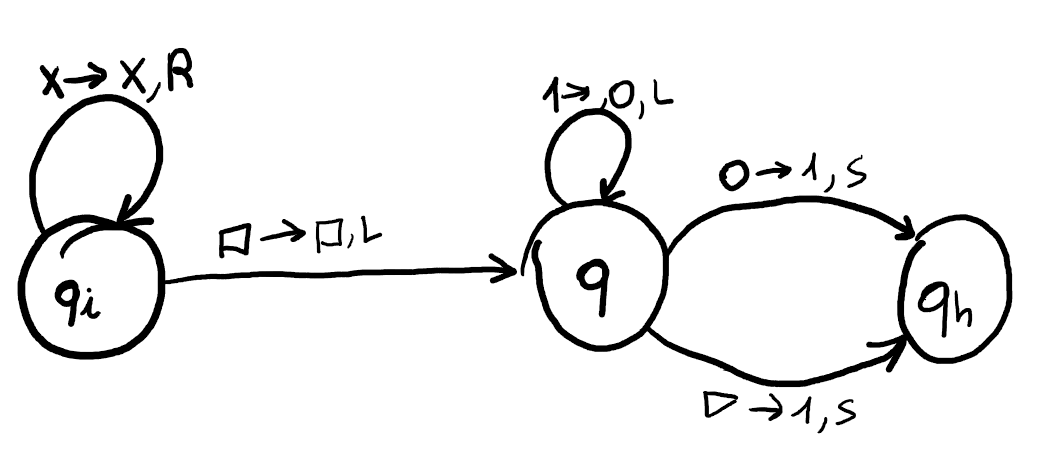
\includegraphics[scale=0.4]{figures/old/TM_increment_1}}
\end{figure}
This will have as alphabet:  \(\Gamma = \{\rhd, 0, 1,  \square\}\) \\
It will have the following states \(\mathcal{Q} = \{q_i, q, q_h\}\) \\
And will have the following transition function:\\
\(\delta (q_i, x) = (q_i, x, R)\)  \\
\(\delta (q_i, \square ) = (q, \square, L)\)  \\
\(\delta (q, 1 ) = (q, 0, L)\) \\
\(\delta (q, 0 ) = (q_h, 1, S)\) \\
\(\delta (q, \rhd ) = (q_h, 1, S)\) \\
Now we need a decrement TM:
\begin{figure}[H]
	\centerline{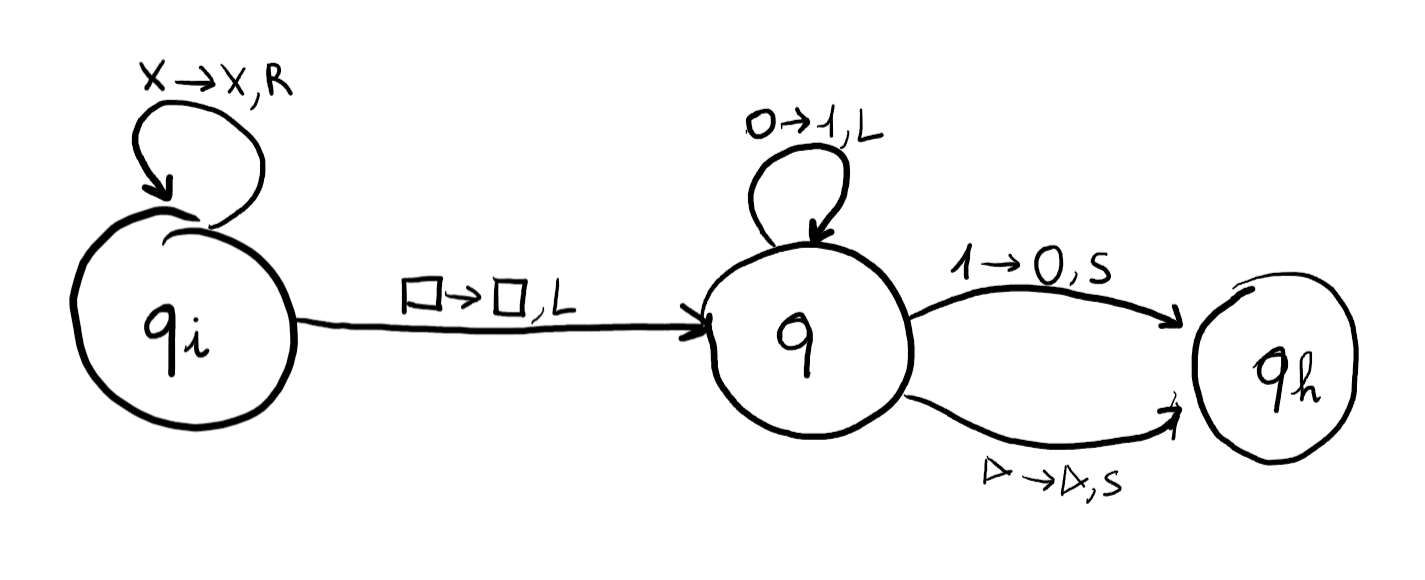
\includegraphics[scale=0.4]{figures/old/TM_decrement_1}}
\end{figure}
This will have as alphabet:  \(\Gamma = \{\rhd, 0, 1,  \square\}\) \\
It will have the following states \(\mathcal{Q} = \{q_i, q, q_h\}\) \\
And will have the following transition function:\\
\(\delta (q_i, x) = (q_i, x, R)\)  \\
\(\delta (q_i, \square ) = (q, \square, L)\)  \\
\(\delta (q, 0 ) = (q, 1, L)\) \\
\(\delta (q, 1 ) = (q_h, 0, S)\) \\
\(\delta (q, \rhd ) = (q_h, \rhd, S)\) \\

So putting all together we will obtain our TM that does the addition of two number. The input will be something like \(...\rhd 010001+0110\square \square...\) .
\begin{figure}[H]
	\centerline{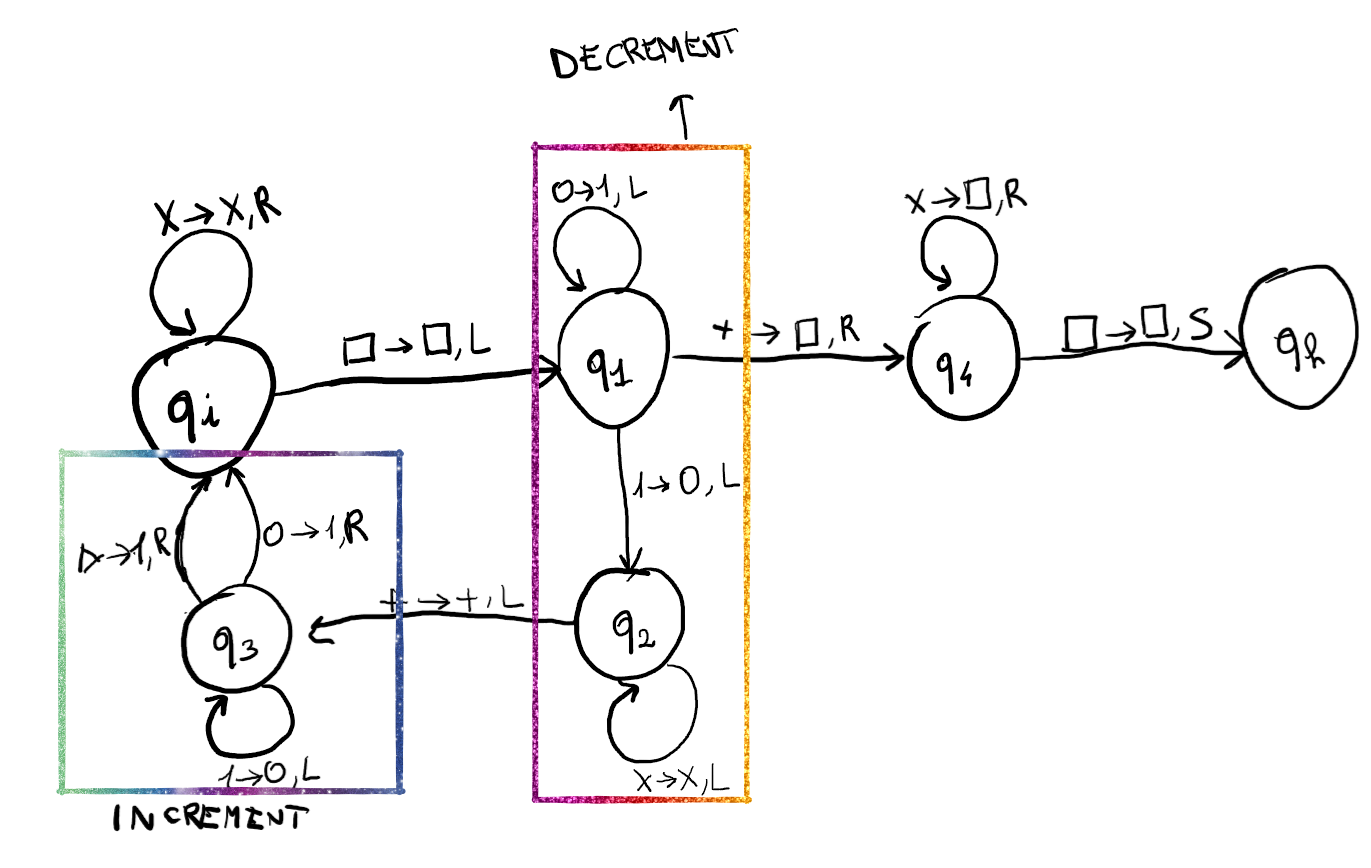
\includegraphics[scale=0.4]{figures/old/TM_addition}}
\end{figure}
This will have as alphabet:  \(\Gamma = \{\rhd, +, 0, 1,  \square\}\) \\
It will have the following states \(\mathcal{Q} = \{q_i, q_1,q_2,q_3,q_4, q_h\}\) \\
And will have the following transition function:\\
\(\delta (q_i, x) = (q_i, x, R)\)  \\
\(\delta (q_i, \square ) = (q, \square, L)\)  \\
... \\

\subsection{Exercise 2}
Write a TM that accept palindromes i.e. write a TM \(\mathcal{M}\) s.t. \(\mathcal{L}(M) = \{w \in \{0,1\}^* | w \text{ is palindrome}\}\) \\
The idea to build this TM is to control if the first and the last digit are equal, if they are equal we substitute them with \(\rhd, \square\) and we continue, if they are different I go into the reject state. If I have an empty string then I can go in the accept state.
\begin{figure}[H]
	\centerline{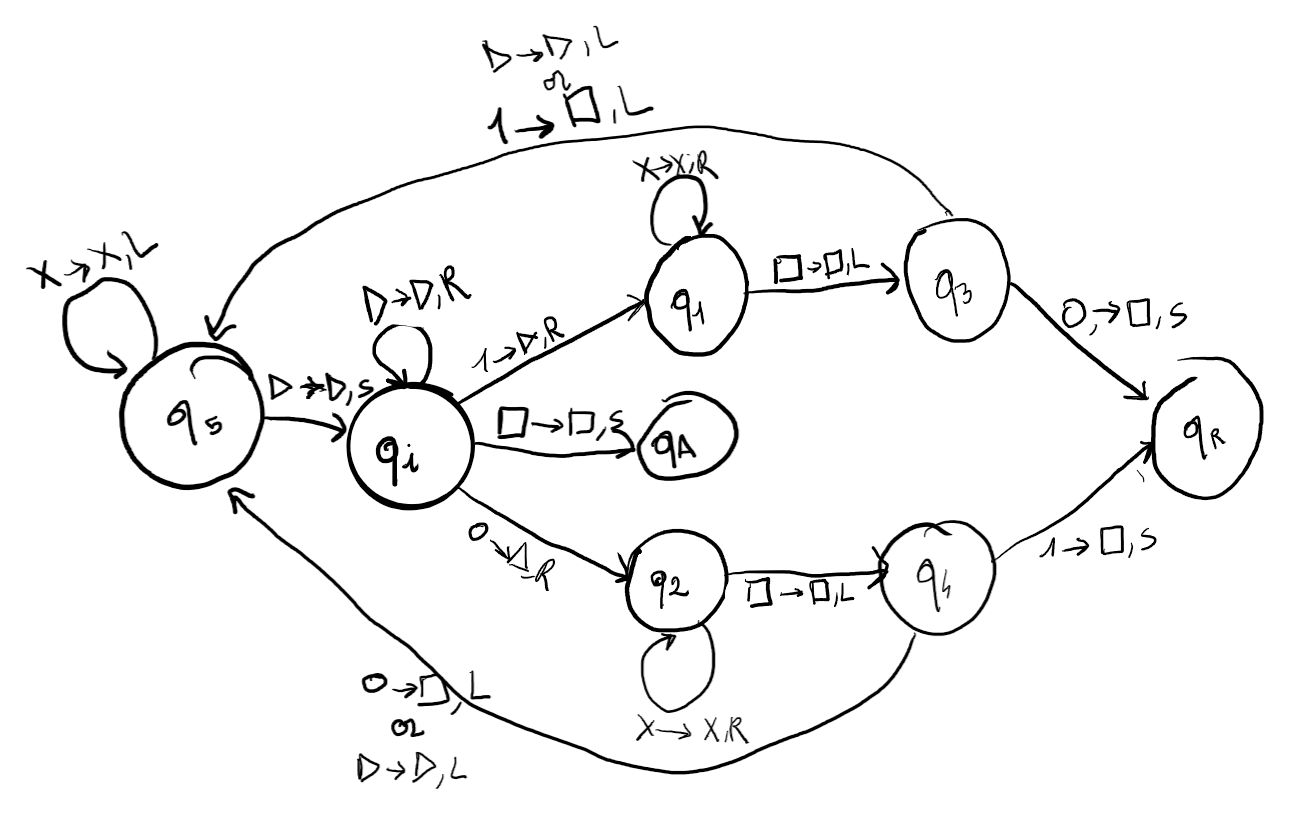
\includegraphics[scale=0.4]{figures/old/TM_palindrome}}
\end{figure}

\subsection{Exercise 3 }
Determine if the following property is \textbf{decidable}:\\
\(P = \{\llcorner N\lrcorner | \mathcal{L}(N) \ infinite \}\) \\
meaning "set of TM so that the languages is infinite.\\
To determine if it is decidable we use the Rice's Theorem. To apply Rice's Theorem we have to prove two things:
\begin{itemize}
	\item P is \textbf{non-trivial}
	\item P is \textbf{extensional}
\end{itemize}
To say that P is \textbf{non-trivial} we have to prove two things:
\begin{itemize}
	\item \(P \neq \emptyset\)
	\item \(\exists N \text{so that }  \llcorner N\lrcorner \notin P\)
\end{itemize}
For the first point we have to prove that exists a TM that accept a language with infinite cardinality:
\begin{figure}[H]
	\centerline{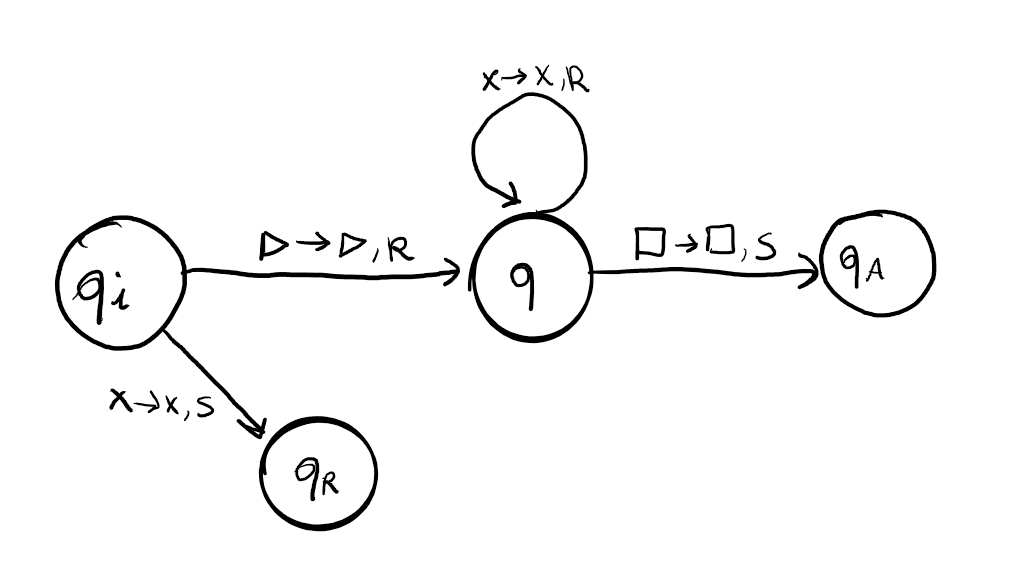
\includegraphics[scale=0.4]{figures/old/TM_always_accept}}
\end{figure}
it never happen that it fails because, the first symbol is always \(\rhd\) .\\
The second thing to prove for P not to be trivial is that exists a TM \(\mathcal{M}\) that does not belong to P:
\begin{figure}[H]
	\centerline{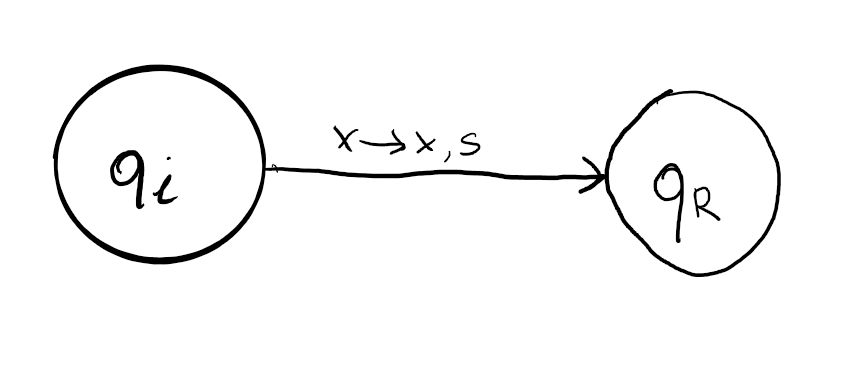
\includegraphics[scale=0.4]{figures/old/TM_always_reject}}
\end{figure}
To say that P is \textbf{extensional} we can say that if we assume that \(\mathcal{L}(M) = \mathcal{L}(N)\) and \(\llcorner M\lrcorner \in P\) we have to show that also \(\llcorner N \lrcorner \in P\). We start by saying that because \(\llcorner M\lrcorner \in P\) iff \(|\mathcal{L}(M)|=\infty\) and we know that   \(\mathcal{L}(M) = \mathcal{L}(N)\), then \(|\mathcal{L}(N)|=\infty\), hence \(\llcorner N \lrcorner \in P\).\\
So from this we can conclude that P is \textbf{undecidable}.

\subsection{Exercise 4 (Construct a TM that decides a language)}
\begin{lstlisting}[breaklines]
Construct a deterministic TM of the kind you prefer, which decides the following language:
L = {w in {0,1}* | between any pair of occurrences of 0 in w there are an odd number of 1s}
Study the complexity of TM you have defined.

solution:
the alphabet is {0,1, start, blank}
the states are {qinit, q1,q2,q3,q4,qa,qr}
the transition function is :
delta (qinit, start) = (q1,start,R)
delta (q1,1)= (q1,1,R)
delta (q1,0)= (q2,0,R)
delta(q1,blank)= (qa, blank, S)
delta(q2, 1)=(q3,1,R)
delta(q2,0)=(q3,0,S)
delta(q2,blank)=(qa, blank,S)
delta(q3, 1)= (q4,1,S)
delta(q3, blank)=(qa, blank,S)
delta(q3,0)= (q2,0,R)
delta(q4, 1)= (q3,1,S)
delta(q4,0)= (qr,0,S)
delta(q4,blank)= (qa, blank, S)

The TM has to go through the tape only one time, so the complexity is linear O(n).
\end{lstlisting}
\begin{figure}[H]
	\centerline{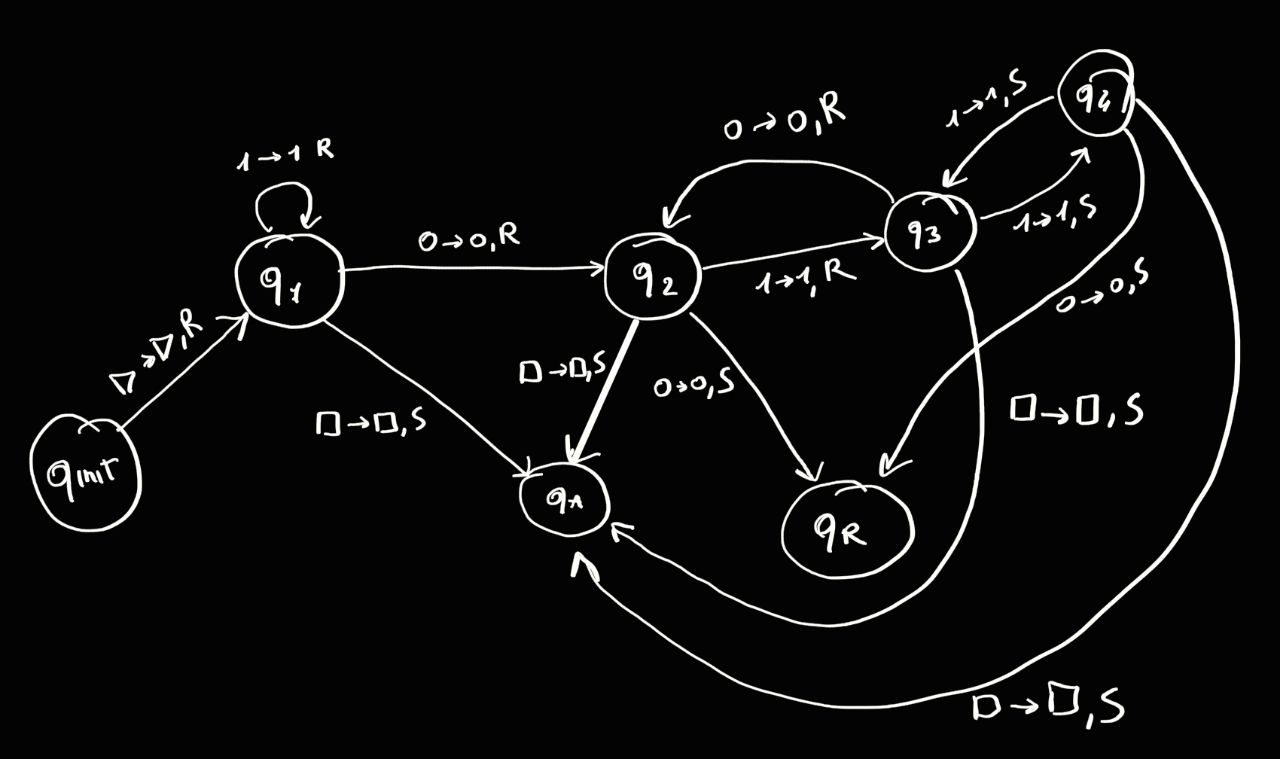
\includegraphics[scale=0.2]{figures/old/TM_1_odd}}
\end{figure}

\subsection{Exercise 5 (Construct a TM that decides a language)}
\begin{lstlisting}[breaklines]
Construct a deterministic TM of the kind you prefer, which decides the following language:
L = {w in {0,1}* | every 1 occurring in w is immediately followed by a 0}
Study the complexity of TM you have defined.
solution 
alphabet: {0,1,start, blank}
states: {qinit, q1,q2,qa,qr}
transition functions:
delta(qinit, start)= (q1,start, R)
delta(q1,0)= (q1,0,R)
delta(q1,1)=(q2,1,R)
delta(q1, blank)=(qa, blank, S)
delta(q2, 0)=(q1,0,R)
delta(q2,1)=(qr,1,S)
delta(q2, blank)=(qr, blank, S)

The complexity of the TM is linear  because it goes through the tape only one time one bit at a time.
\end{lstlisting}
\begin{figure}[H]
	\centerline{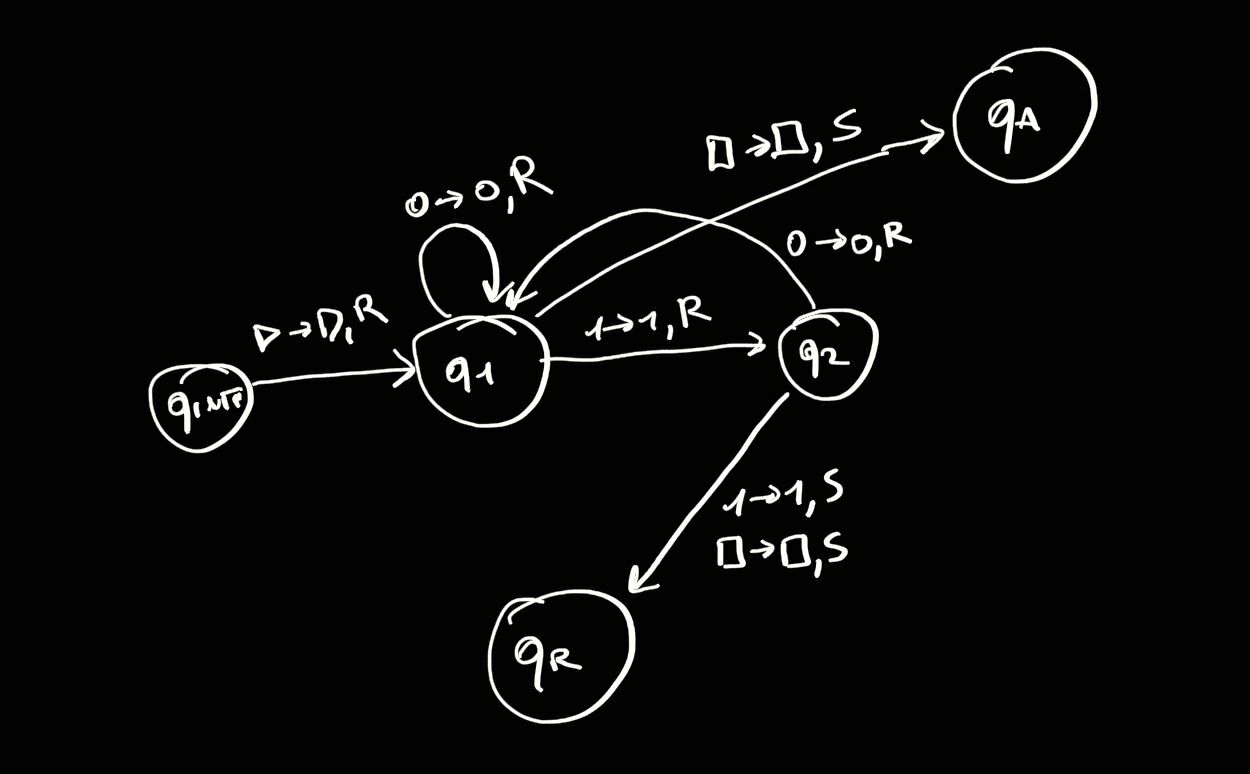
\includegraphics[scale=0.2]{figures/old/TM_2}}
\end{figure}
\subsection{Exercise 6 (Construct a TM that decides a language)}

\begin{lstlisting}[breaklines]
Construct a deterministic TM of the kind you prefer, which decides the following language:
L = {w in {0,1}* | does not contains 10 as substring}
study the complexity of the TM you have defined.

solution:
alphabet: {0,1,start, blank}
states: {qinit, q1,q2,qa,qr}
transition function :
delta(qinit, start)= (q1, start, R)
delta(q1,0)= (q1, 0,R)
delta(q1, 1)=(q2,1,R)
delta(q1, blank)=(qa, blank,S)
delta(q2,0)=(qr,0,R)
delta(q2,1)=(q2,1,R)
delta(q2, blank)=(qa, blank,S)

This TM decides the language in polynomial time, in fact it goes through the tape only one time, one symbol at a time. In particular it is linear, DTIME(n) where n is the size of the input string.
\end{lstlisting}

\section{Exercises 2}

\subsection{Exercise 1}
\textbf{Prove that a problem is in P}\\
Given a list \(A = [a_1,...,a_n]\) s.t. \(\forall i \  a_i \in N \) return an index \(i \in \{1,...,n\}\) s.t. \(A[i] = v\), where \(v \in N\), if any, otherwise return -1. \\
So here we have as input a list A and a natural number v. The result will be a natural number. \\
\textbf{Solution}\\
1. \textbf{Give a pseudo-code}:
\begin{minted}[style=fruity, bgcolor=black]{python}
i <- 1 
while i < n do {
if A[i] == v return i
else i <- i +1
}
return -1

\end{minted}
2. \textbf{encode the input of the program as bit string}, and show that it can be done in polynomial time:\\
We know that if I want to encode a natural number n I will need a number of bit that is \(log(n)+1\). One possible way to encode a list of natural number is to separate them by a symbol ($\#$) so that now our alphabet will have 3 symbols (0, $\#$,1) that will be encoded in binary as (00,01,11). So now to encode a natural number we will need \(2 \cdot (log(n) +1)\) bit, so the total length of the encoding of the input will be :
\[l = |\llcorner (A,v)\lrcorner| = (\sum_{i=1}^n 2 \cdot (log(a_i) +1)) + 2n+ 2(log(v) +1\]
3. \textbf{Prove that the number of basic instructions of our pseudo-code is bounded by a polynomial in l}\\
In our pseudo-code we have :
\begin{itemize}
	\item 1 assignmente
	\item n iteration (in the worst case)
	      \begin{itemize}
		      \item 1 inequality check
		      \item a conditional branching
		      \item 1 equality check
		      \item 1 addition
		      \item 1 assignment
	      \end{itemize}
	\item a return instruction
\end{itemize}
So I have n iteration in which we do c number of instruction and out of the iteration we have b number of instruction so the total number of instruction is: \(b+n\cdot c \leq p(l)\), meaning that can be bounded by a polynomial in l.\\
4.\textbf{All intermediate results are polynomially bounded in length}\\
i start by 1 and we add 1 for n times so i is polynomially bounded.\\
5. \textbf{Argue that each instruction can be simulated by a turing machine that runs in polytime with respect to l}\\
All the operation done in our code can be simulated by a TM that runs in polytime
\begin{itemize}
	\item assignment
	\item inequelity check
	\item equality check
	\item adding 1
\end{itemize}

\subsection{Exercise 2 (Prove a function to be in FP)}
\begin{lstlisting}[breaklines]
You are required to prove that the following function f in in FP. To do that, you can give a TMs or define some pseudocode. The function is one that, given two strings v,w checks wheter v is a substring of w, namely wheter w contains an exact occurrence of v.

solution:
1. pseudo-code:
n = size(w);
m=size(v);
k=0
 for i in 0..n-1
  if (v[k]==w[i]){
    k++
   }
   else {
   k=0
   }
   return k==m
   
   
2. encode the input as a bit string:
   given n the number of different symbols in the string v and w, we need (log n +1) bit for every symbol, we also need a separation symbol # between characters and a separation symbol between the two string @, so the alphabet {0,1,#,@} will be encoded as {00,01,11, 10} so we need, given k=size(v)+size(w) we have the total size of the encoded input will be:
   size(input) = 2k(log n +1)+ 2k + 2 that is polynomial.

3. number of basic instruction:
-assignment
-assignment
-assignment
-loop 
 -equality check
  -add 1 and assignment
 -assignment
-equality check
so the number of instruction will be a+bn= O(n), where n<size(input) so the number of basic instruction is polynomial with respect to the seize of the input.

4. All intermediate result are bounded polynomially in length:
 k goes from 0 to the size of v and i goes from 0 to the size of w.
 
 5. argue that every instruction can be simulated by a TM that runs in polyomial time:
 We have only assignment, addition of 1 that can be done in polytime by a TM and equality check that can be done in polytime.
\end{lstlisting}

\subsection{Exercise 3 (prove a function to be in FP)}
\begin{lstlisting}[breaklines]
You are required to prove that the following function f is in FP. To do that you can give a TMs or define some pseudocode. The function is one that, given a list L=L1,...,Ln, returns its inverse namely Ln,Ln-1,...,L1.
solution:
1. Pseudocode:
k = size(L)
j = 0 
for i in k-1 to 0
 Inv_L [j] = L[i]
 j++
return Inv_L

2. encoding of the input:
The input is a list so the encoding will be the encoding of each element separated by a symbol  #. We do not know what L1,...,Ln but let's say that they are natural number in this case the encoding would be L1#L2#...#Ln, the alphabet would be {0,1,#}, in bit would be {00,01,11}, so the total length would be 2n(log L +1)+ 2n.
3. number of basic instruction:
The number of basic instruction will be c+ n*a so O(n), where n is the size of the input.
4. each instruction can be simulated by a TM: We can simulate each instruction by a TM, we have assignment, addition of 1 and equality check that can be done in polynomial time by a TM.
5. All data used is polynomial in the input: 
  -k is the size of the input
  -j start from 0 and add 1 for k time, so it will have value k
  -Inv_L has the same size as the input
\end{lstlisting}

\subsection{Exercise 4 (prove a function to be in FP)}
\begin{lstlisting}[breaklines]
You are required to prove that the following function f is in FP. To do that, you can give a TMs or define some pseudocode. The function is one that, given two lists L=L1,...,Ln and P = P1,...,Pn of rational numbers returns their scalar products.

solution:
1. pseudocode
n=size(P)
dot = 0
for i in 0..m
dot = dot + L[i]*P[i]
return dot

2. encode the input 
The input is formed by two list of rational numbers. we need a symbol to separate the two list @, we need a symbol to separate the rational numbers #, a symbol to separate the numerator from the denominator / and and two symbols for the sign so that in total we would have the following alphabet {+,-,0,1,#,@} so we would need 3 bit. we encode the rational number as Sign num/den, where num and den are natural numbers, and so they would need log k +1 bit. In total we would have : 3*2*2*n(log n+1)+ 3*2*n+ 3 that is polynomial.
3. number of basic instruction is polynomial
the number of basic instruction is c+n that is polynomial in the input encoding length
4. each instruction can be simulated by a TM working in poly time: as basic instruction we have assignment, sum, multiplication that could be done in polynomial time.
5. all data used is polynomial in the size of the input:
dot is a natural number, its size is polynomially bounded by the size of the input.
\end{lstlisting}



\section{Exercises 3}
\subsection{Exercise 1}
Suppose clique is the following set: \[\text{CLIQUE} = \{(\mathcal{G}, k) \ | \ \text{ is an undirected graph containing a glique of size at least k }\}\]\\
\textbf{Prove that clique is NP-complete} by showing that \(3SAT \leq_p \text{CLIQUE}\)\\
\textit{Hint: consider any 3CNF F as a graph whose vertices are the occurrences of literals in F}
\\
\textbf{Solution}
A clique is a subset \(W \leq V\) of its vertices such that any pair \(v,w \in W\) of distinct vertices is such that \(\{v,w\} \in E\) . In other words given an undirected graph a clique is a subset of this graph where all the vertices are connected.
\begin{figure}[H]
	\centerline{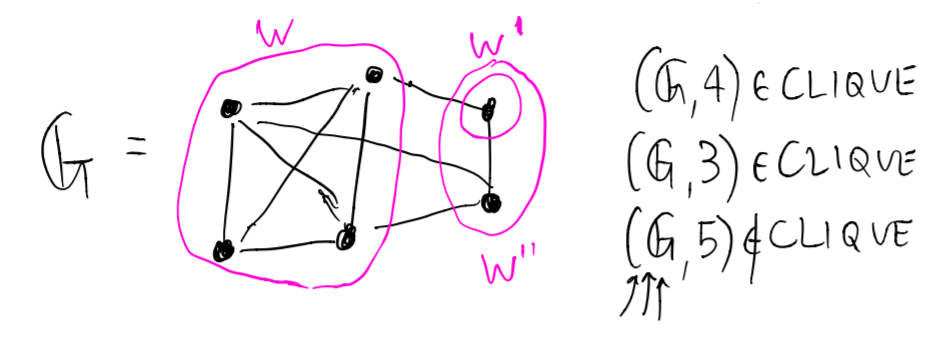
\includegraphics[scale=0.4]{images/clique}}
\end{figure}
So \((\mathcal{G},4)\) belong to clique because in w (pink) I can see that I have at least 4 vertices which are all connected.  \((\mathcal{G},5)\) does not belong to clique because I can't find a subset of the graph where 5 vertices are all connected.\\
The fact that clique in in NP is easy to prove: the certificate, as expected, is a subset \(W \subseteq V\) such that \(W\) has a k-CLIQUE. Indeed:
\begin{itemize}
	\item Its size (which is its cardinality) is smaller than the one of \(\mathcal{G}\).
	\item checking that \(W\) is indeed a clieque of size \(\geq\) to k can be done in quadratic time: it sufficies to check that any pair of distinct vertices \(v,w \in W\) are connected by an edge.
\end{itemize}
About completeness, we want a reduction \(f\) such that for every 3CNF F, \(f(F)\) is a pair \((\mathcal{G}, k)\), and moreover \((\mathcal{G}, k) \in \text{CLIQUE}\) IFF F is satisfiable. So first of all we can observe that a natural way of turning CNFs into graphs consist in introducing a node for each literal in the CNF. So let's see what it means graphically
\begin{figure}[H]
	\centerline{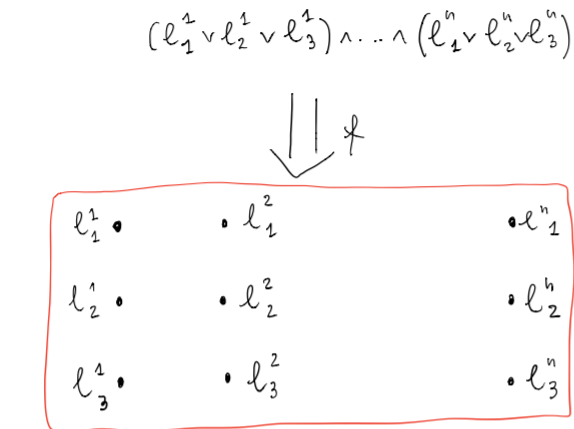
\includegraphics[scale=0.4]{images/clique_1}}
\end{figure}
for every \(i \ne j\) and for every \(s,q \ in \{1,2,3\}\) we have an edge beween \(l_s^i\) and \(l_q^j\) iff the two literals are compatible from a logical point of view, namely iff they don't talk about the same variable in inconsistent ways (for example, we do not have an edge between \(x\) and \(\lnot x\) . \\
The only missing ingredient in the proof is to prove that F is satisfiable IFF \(f(F)\) has a CLIQUE of size equal to the number of clauses in F:
\begin{itemize}
	\item Suppose that F is satisfiable, then there is an assignment of truth value to the variables in F which makes the n clauses of F all \textbf{true}. This means that for every \(i \in \{1,...,n\}\) (the clause) there exists \(s \in \{1,2,3\}\) (the literals inside each clause) such that \(l_s^i\) is true in the assignment. All this literals then are pairwise consistent (i.e. it can't be that \(l_s^i=x \text{ and } l_q^j =\lnot x\) ), the nodes corresponding to these literals in \(f(F)\) are all linked by an edge. Hence \(f(F)\) is indeed a graph which has a clique of size n.
	\item Suppose that the graph \(f(F)\) has a clique of size n. It means that all columns of \(f(F)\) are "involved" in the clique (because there are no edges between nodes in the same column). There is thus a way of choosing for each clause in F one of its literals in such a way as to preserve logical consistency, and this, by definition of logical consistency, means that there is an assignment which makes all these literals true, since we have at least one literal for each clause. The formula F is satisfiable.
\end{itemize}

\subsection{Exercise 2 (prove a language to be in NP)}
\begin{lstlisting}[breaklines]
You are required to prove that the following problem L in in NP. To do that, you can give a TM or define some pseudocode. The language L includes precisely those binary strings which are encodings of pairs in the form (G,t) where G is a graph and t is a natural number, such that the nodes of G can be partitioned into at most t sets in such a way that nodes which are part of distinct sets are not linked by any edge.
 or equivalently:
 You are required to prove that the following problem L in in NP. To do that, you can give a TM or define some pseudocode. The language L includes precisely those binary strings which are encodings of pairs in the form (G,k) where G is a graph and k is a natural number, such that the nodes of G can be assigned a natural number between 1 and k in such a way that nodes which are linked by an edge are assigned distinct natural numbers.
 
Solution:
L = {(G,k) | exists N, if (u,v) belong E, N[u]!=N[v] }
where G = (V,E)
-CERTIFICATE: We take as a certificate N, list of natural number assigned to each node of G.
-CERTIFICATE SIZE: N is a list of size |V| of natural number <k. So the certificate size is O(|V| * log(k) ) , which is polynomial in the size of the input.
-TM FOR CHECKING THE CERTIFICATE (VERIFIER): The TM will have to check if every pair in E has different values in N. So:
	for (u,v) in E
    	if (N[u]==N[v])
         return false
    return true
    
    this has a complexity O(|E|)=O(|V|^2) which is polynomial.
    
    So L is in NP.
   
\end{lstlisting}
\subsection{Exercise 3 (1SAT)}
\begin{lstlisting}[breaklines]
Consider the following problem:
1SAT = {A|A is a satisfiable 1CNF}
To which complexity class does 1SAT belong? Prove your claim.

Solution:
1SAT belong to the complexity class P.
prove:
1. Pseudocode:
n = size(A)[0]
for i in 0..n
 for j in 0..n
   if (A[i][0]==A[j][0] and A[i][1]!=A[j][1])
    return false
return true
2. Encoding of the input:
the input can be encoded as a list of literals, that can be negated or not. We will need a symbol to separate the literals, one to negate a literal so in the end we will have the following alphabet {0,1,#,@} that encoded will be {00,01,10,11}. If k is the number of different literal and n the total number of literals and w is the total number of negated literal w<n, we will have that the total length of the input encoding will be l= 2 (n(log k +1)+ n+ w) that is polynomial in the length of the input.
3. number of basic instruction:
The number of basic instruction is c+b*n^2 which is polynomially bounded with respect to the length of the encoding of the input.
4. basic instruction polynomially bounded with respect to the length of the input encoding:
every instruction can be modeled by a TM that works in polynomial time, equality check, infact, can be done in polynomial time by a TM.
5. Every partial result is polynomially bounded by the length of the input encoding:
i is a natural number that goes from 0 to the size of the input, so it is polynomially bounded.

Follow that 1SAT is in P.
\end{lstlisting}
\subsection{Exercise 4 (ONEINDSET)}
\begin{lstlisting}[breaklines]
We studied the problem INDSET. You are required to classify the subset ONEINDSET of INDSET whose elements are pairs G,k, such that G is an undirected graph such that every node is contained in at most one edge, and k is a natural number. To which complexity class does ONEINDSET belong?

solution:
definition of ONEINDSET 
Input: (G,k)
Output: 1 iff exists I subset V s.t. |I| >=k and for u,v in I then (u,v) not belong to E and for every u s.t exists u,v in E then not exists u,w in E, v!=w.

I can try to prove that ONEINDSET is in P:
Theorem: Let G=(V,E) be an undirected graph. If every v in V is contained in at most one edge then G has an independent set of size |I|=|V|-|E| .
 prove: if I have that every v in V is contained in at most one edge then if I have a pair (u,v) in E then they will not be in any other pair. So I Will have two independent set of size |V|-1, if I apply this for every pair in E, I will have an independent set of size |V|-|E|.
 This theorem allow us to build a simple TM deciding ONEINDSET that trivially works in polynomial time, therefore ONEINDSET is in P.
\end{lstlisting}

\subsection{Exercise 5 (THREECLIQUE)}
\begin{lstlisting}[breaklines]
We studied the problem CLIQUE. You are required to classify the subset THREECLIQUE of CLIQUE consisting of all the pairs (G,3). To which class does THREECLIQUE belong?

solution:
THREECLIQUE belong to the class P.
1. Pseudocode
for i in V
 for j in V
  for k in V
   if (i,j) in E and (i,k) in E and (j,k) in E
    return true
  return false
2. encoding the input
The input is G=(V,E). V can be encoded as a natural number, while E as pairs of natural numbers. We need a symbol # to separate the different natural numbers so our alphabet will be {0,1,#} that encoded will be {00,01,11}. The total bits that we need will be:
l= 2(2*|E|(log(n)+1) + 2|E| + (log V +1) +1)= O(|E|)= O(|V|^2)
3. number of basic instruction:
we have three innested loop from 1 to V, so the total number of instruction is c+b|V|^3= O(|V|^3) which is polynomial in the length of the encoding of the input.
4. basic instruction TM polynomially bounded
The only non-trivial instruction is checking if a pair is connected by an arc, which can be done in O(|E|)=O(|V|^2) = O(l) which is polynomial with respect to the size of the encoding of the input.
5. partial data polynomially bounded 
i,j,k are natural number, their maximum size will be (log |V| +1) bit which is polynomially bounded with respect to the size of the encoding of the input.
\end{lstlisting}
\subsection{Exercise 6 (4SAT)}
\begin{lstlisting}[breaklines]
4SAT = {A | A is a satisfiable 4CNF}
to which complexity class does 4SAT belong? Prove your claim.

solution:
4SAT is NP-Complete.
 -4SAT is in NP
 4SAT = {A | exist P such that A(P)=true}
 P is the certificate and it is an assignment for every variable so its length it's polynomial with respect to the length of A. 
 The TM that has to verify, has to substitute the values of thruthness in A, and this can be done in polynomial time. 
 So 4SAT is in NP.
 -I can reduce 4SAT from 3SAT -> 3SAT <=_p 4SAT
 definition:
  3SAT:
   input: A
   output 1 iff A is satisfiable and 3CNF
 
 4SAT:
  input:A
  output 1 iff A is satisfiable and 4CNF
  
  3SAT <=_p 4SAT means that A in 3SAT iff M(A) in 4SAT  
For each clause of the type (A or B or C) I create two claused of the type (A or B or C or D) and (A or B or C or notD), this way the truth value of D becomes irrelevant to the satisfiability of the 4CNF. The reduction is polytime because I just add a new variable for each clause.
  - for the statement 3SAT =>4SAT, since we created a new variable that for construction is irrelevant, then if a (A or B or C) is true then also (A or B or C or D) and (A or B or C or notD) is true.
  -for the statement 4SAT =>3SAT if I have that (A or B or C or D) and (A or B or C or notD) is satisfiable, since we have bot D and notD in different clauses it is irrelevant. So without D the formula will be satisfiable in 3SAT.
\end{lstlisting}

\subsection{Exercise 7 (2SAT)}
\begin{lstlisting}[breaklines]
Consider the following problem:
2SAT = {A|A is a satisfiable 2CNF}
To which complexity class does 2SAT belong? Prove your claim.

Solution:
This is a quite complex problem to solve, but it has been solve and 2SAT belong to P. The dimonstration is based on the fact that I can rewrite (A or B) as ((notA => B) and (notB => A))
\end{lstlisting}

\subsection{Exercise 8 ( NODECOVER reduction)}
\begin{figure}[H]
	\centerline{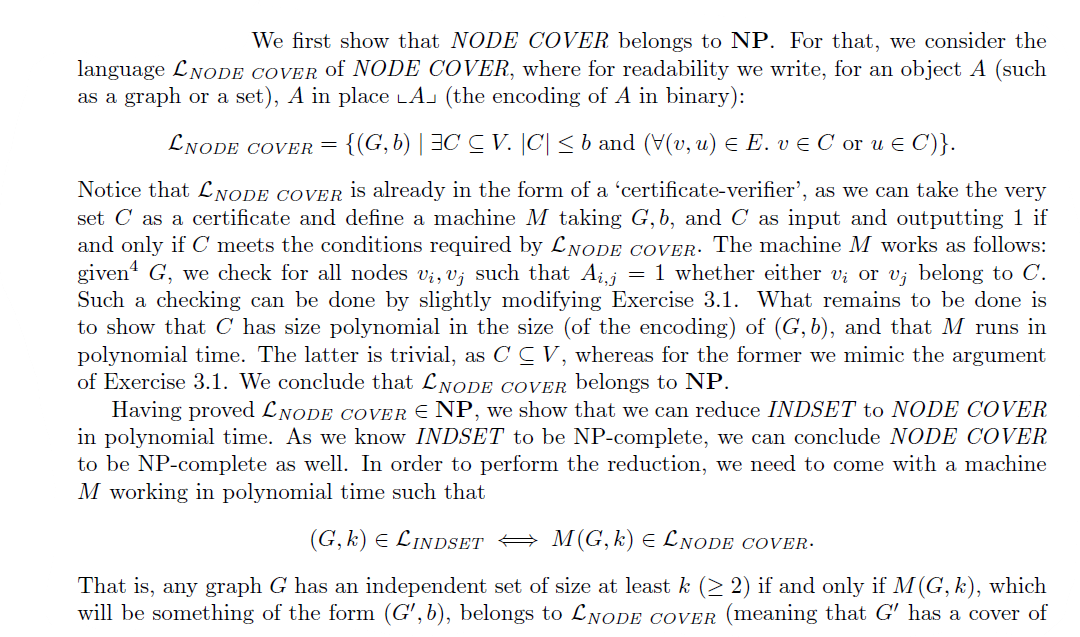
\includegraphics[scale=0.8]{images/Nodecover1}}
\end{figure}
\begin{figure}[H]
	\centerline{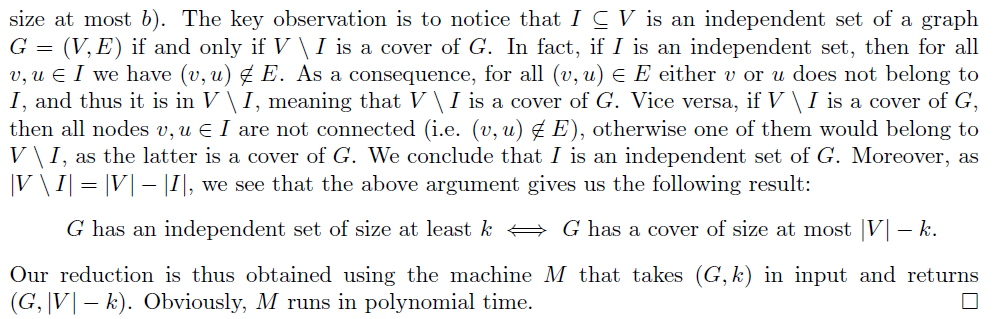
\includegraphics[scale=0.8]{images/Nodecover2}}
\end{figure}
\subsection{Exercise 9 ( SET PACKING reduction)}
\begin{figure}[H]
	\centerline{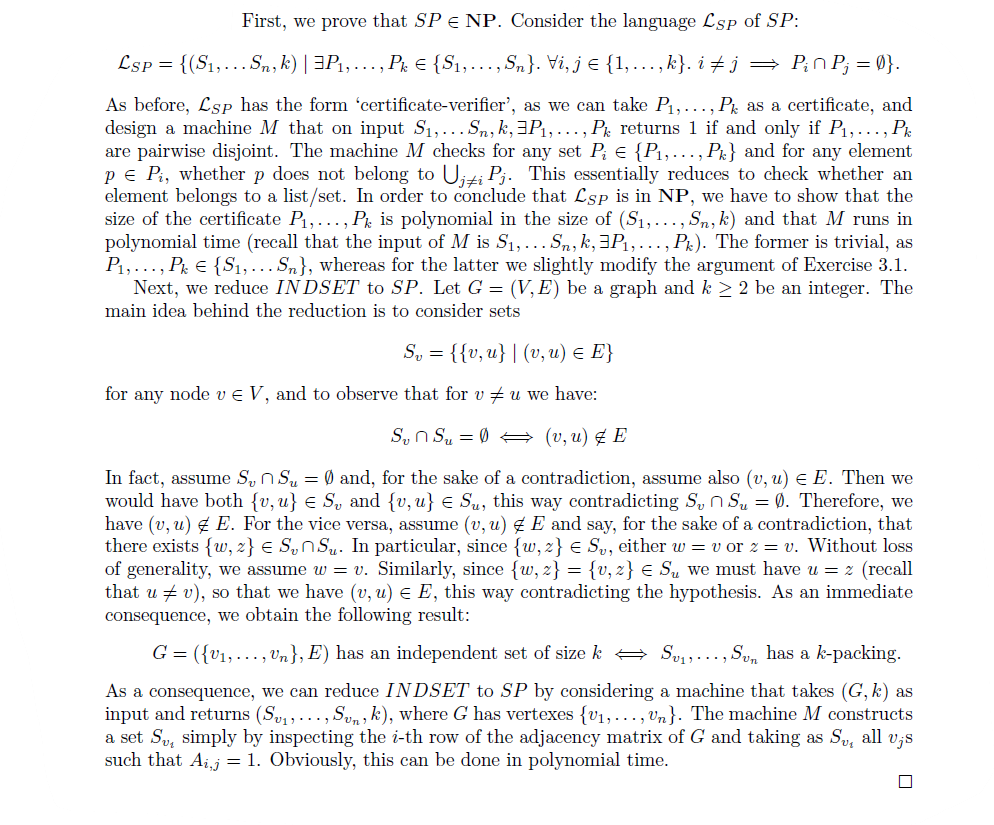
\includegraphics[scale=0.8]{images/SP}}
\end{figure}

% \section{Theory exercises (with solutions)}
%  \begin{figure}[H]
% \centerline{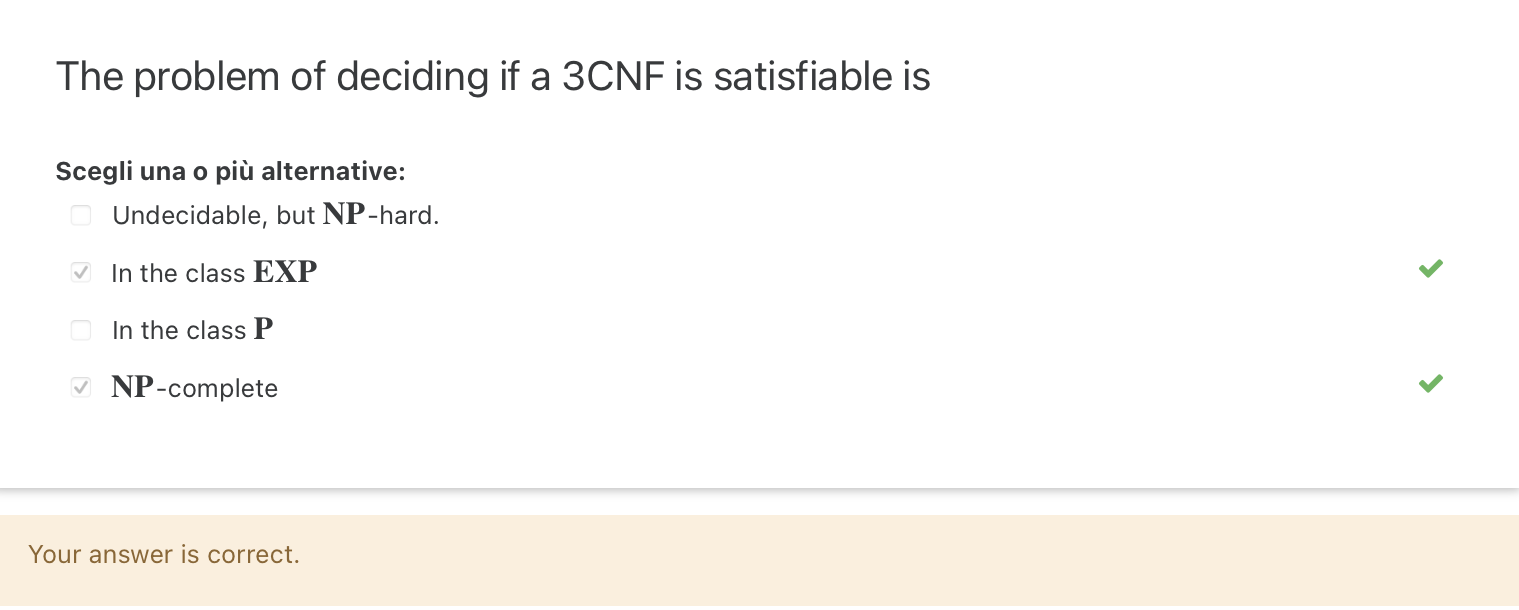
\includegraphics[scale=0.5]{figures/old/theory/1}}
% \end{figure}
%  \begin{figure}[H]
% \centerline{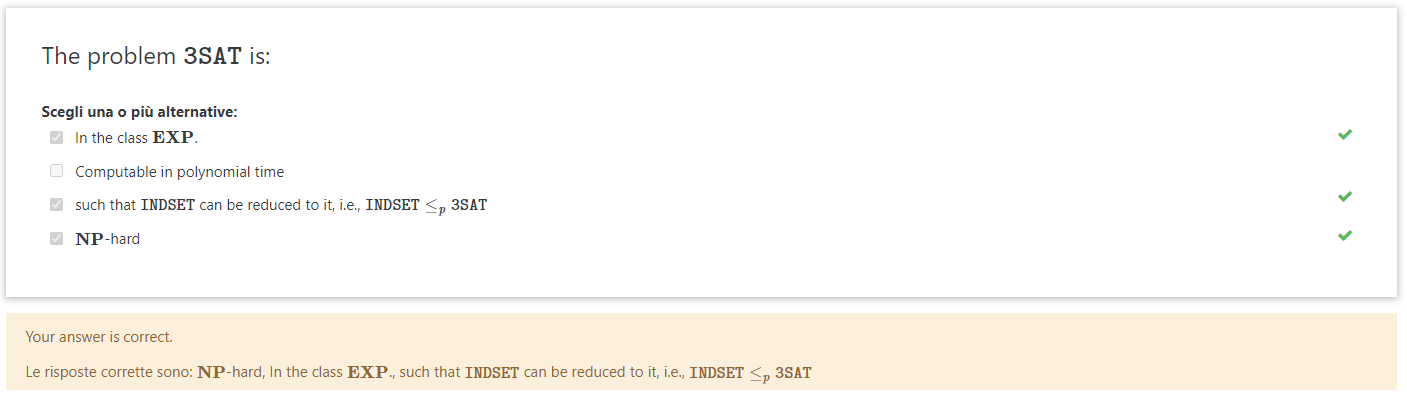
\includegraphics[scale=0.5]{figures/old/theory/2}}
% \end{figure}
%  \begin{figure}[H]
% \centerline{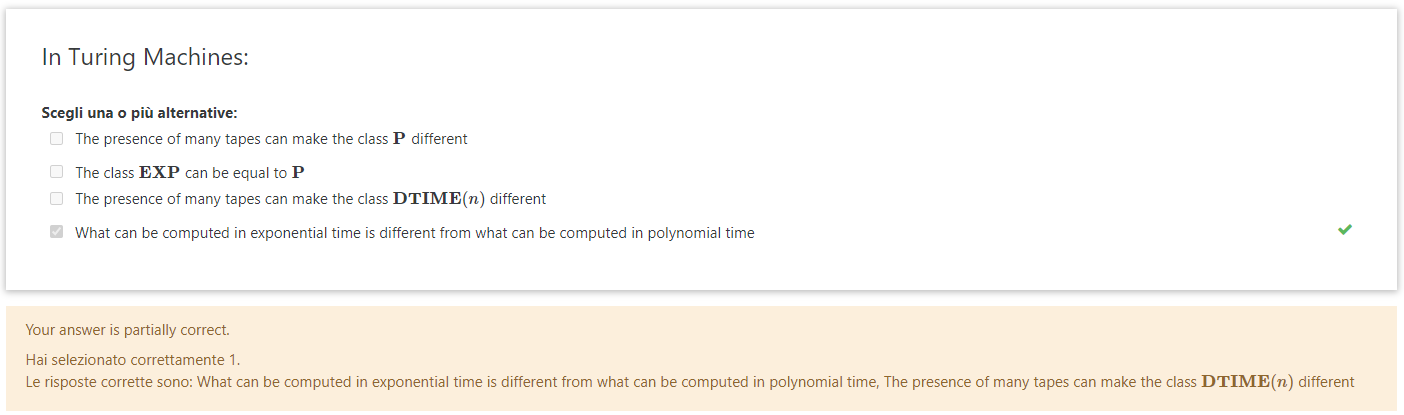
\includegraphics[scale=0.5]{figures/old/theory/3}}
% \end{figure}
%  \begin{figure}[H]
% \centerline{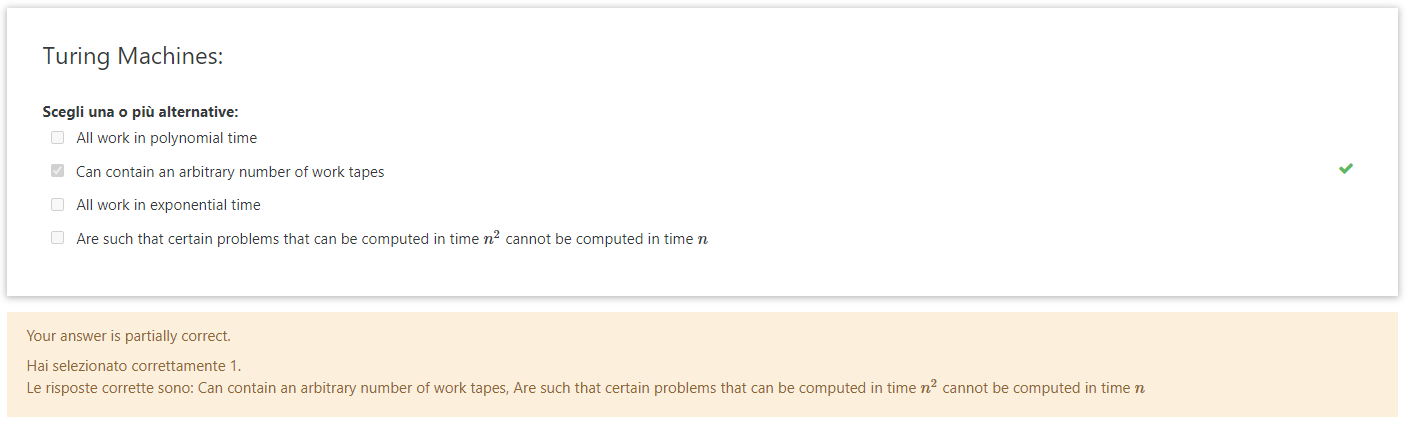
\includegraphics[scale=0.5]{figures/old/theory/4}}
% \end{figure}
%  \begin{figure}[H]
% \centerline{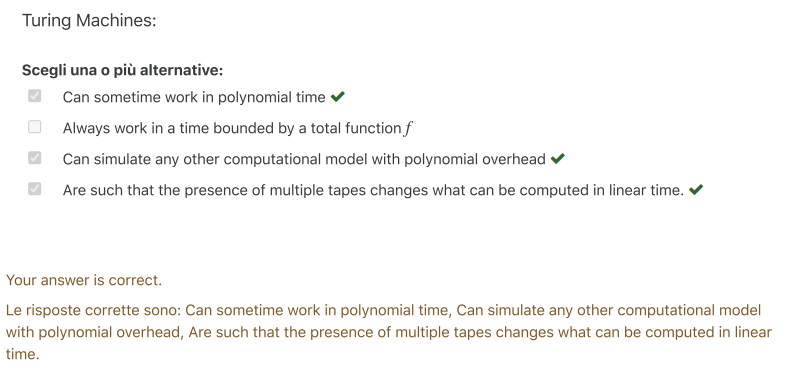
\includegraphics[scale=0.5]{figures/old/theory/5}}
% \end{figure}
%  \begin{figure}[H]
% \centerline{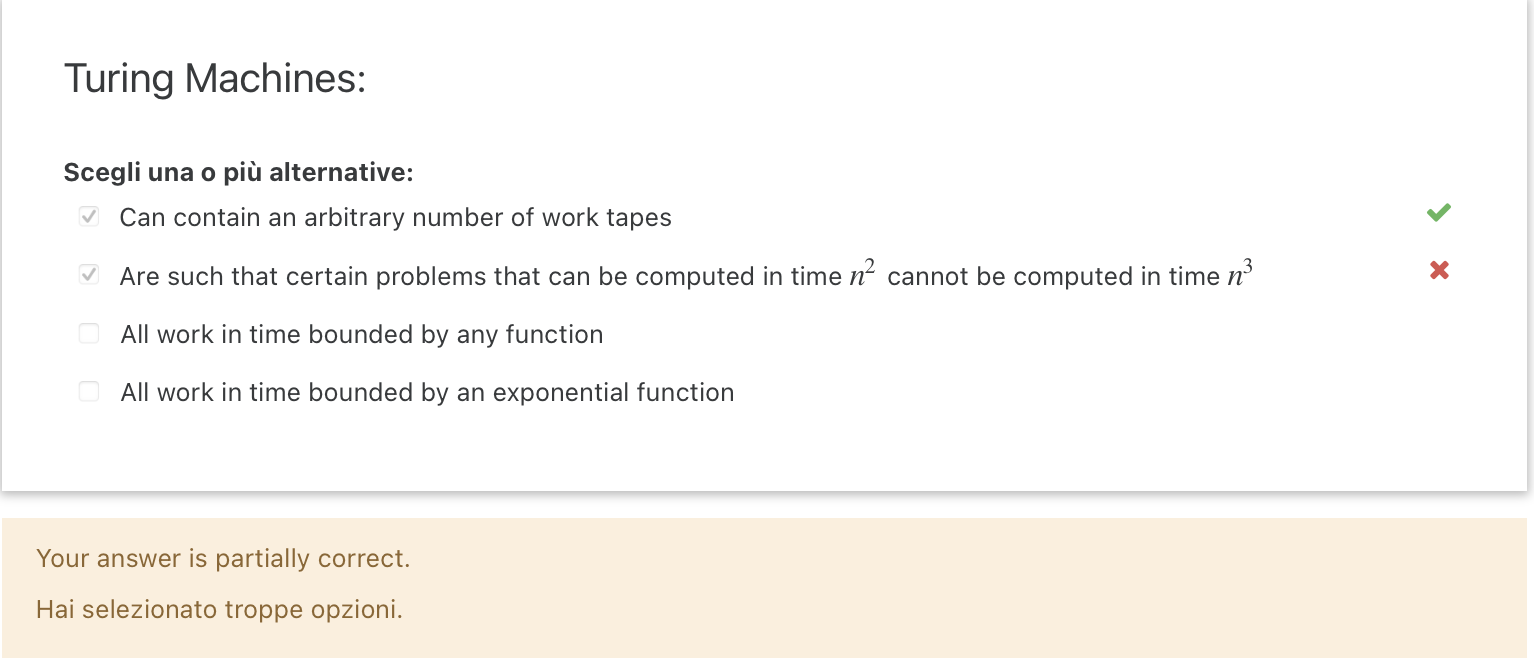
\includegraphics[scale=0.5]{figures/old/theory/6}}
% \end{figure}
%  \begin{figure}[H]
% \centerline{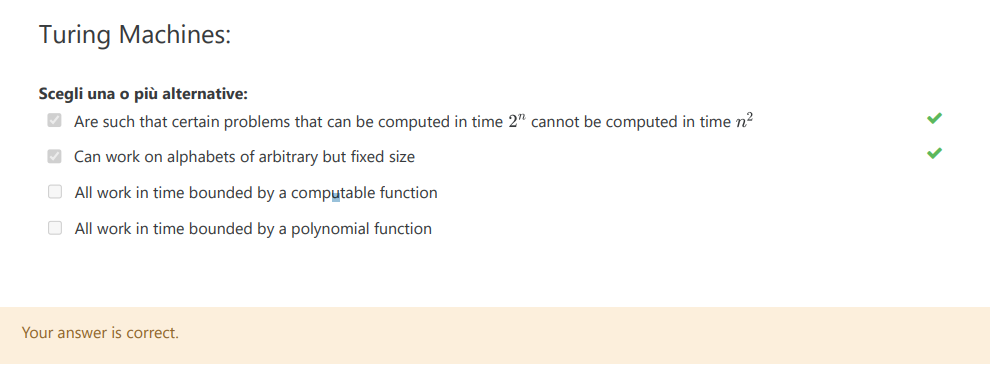
\includegraphics[scale=0.5]{figures/old/theory/7}}
% \end{figure}
%  \begin{figure}[H]
% \centerline{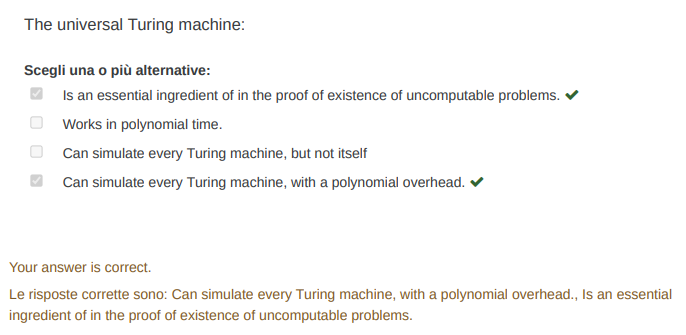
\includegraphics[scale=0.5]{figures/old/theory/8}}
% \end{figure}
%  \begin{figure}[H]
% \centerline{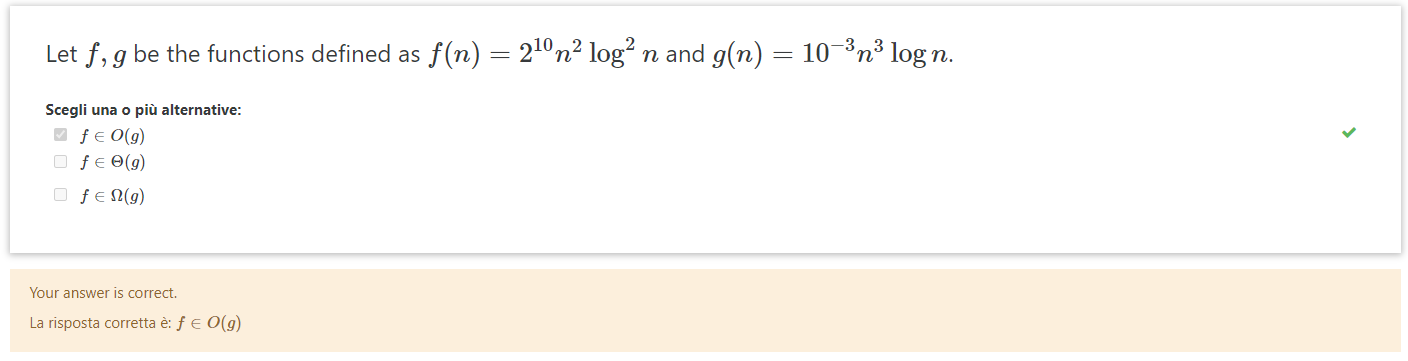
\includegraphics[scale=0.5]{figures/old/theory/9}}
% \end{figure}
%  \begin{figure}[H]
% \centerline{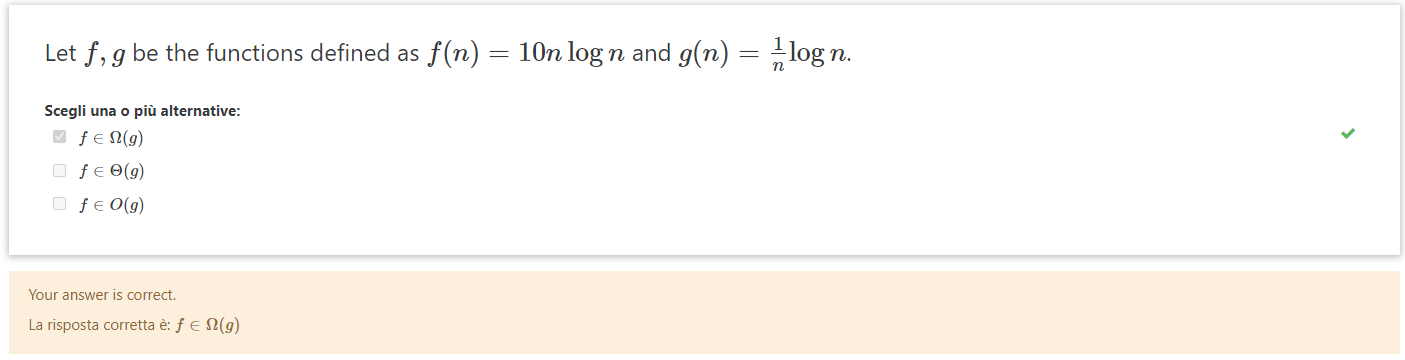
\includegraphics[scale=0.5]{figures/old/theory/10}}
% \end{figure}
%  \begin{figure}[H]
% \centerline{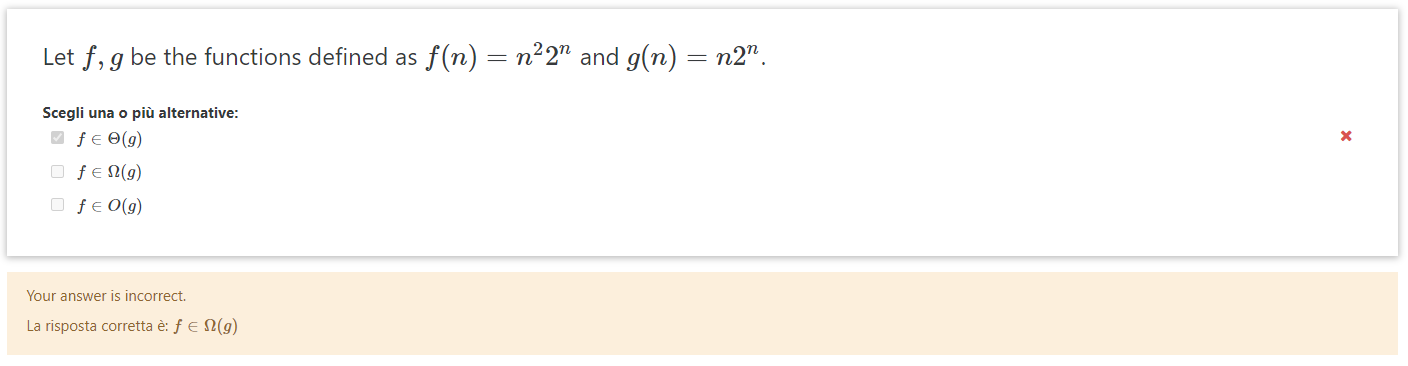
\includegraphics[scale=0.5]{figures/old/theory/11}}
% \end{figure}
%  \begin{figure}[H]
% \centerline{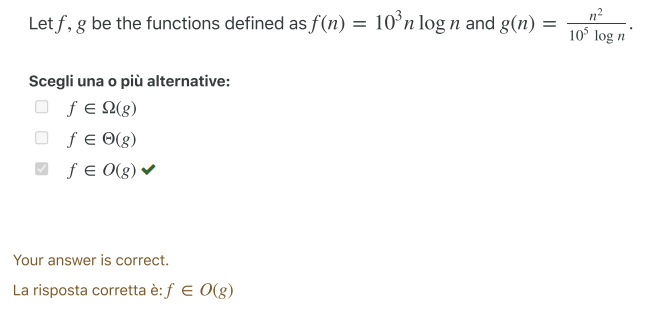
\includegraphics[scale=0.5]{figures/old/theory/12}}
% \end{figure}
%  \begin{figure}[H]
% \centerline{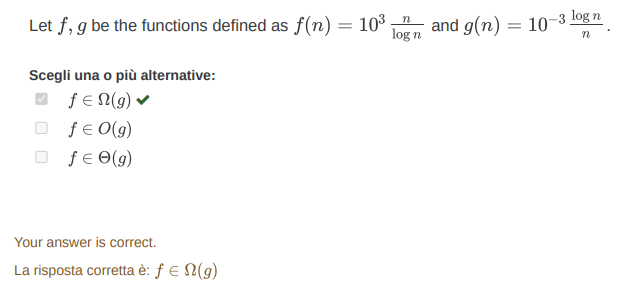
\includegraphics[scale=0.5]{figures/old/theory/13}}
% \end{figure}
%  \begin{figure}[H]
% \centerline{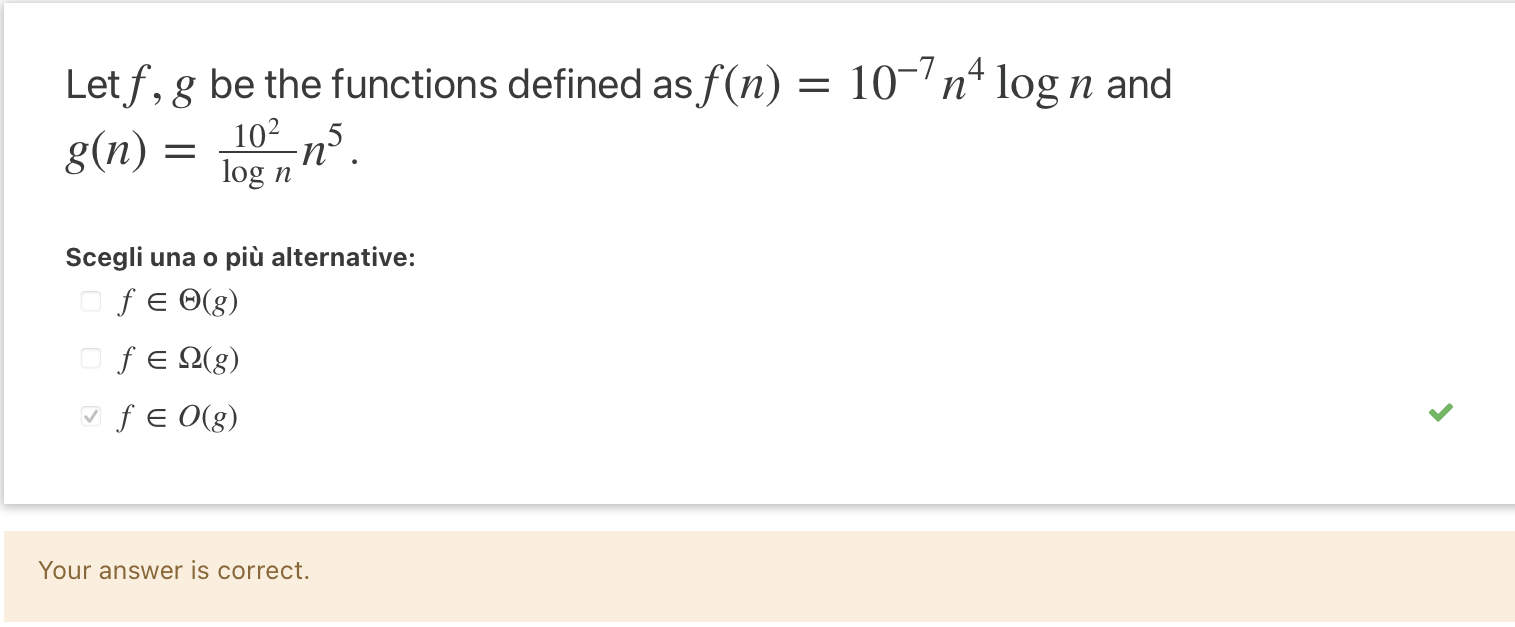
\includegraphics[scale=0.5]{figures/old/theory/14}}
% \end{figure}
%  \begin{figure}[H]
% \centerline{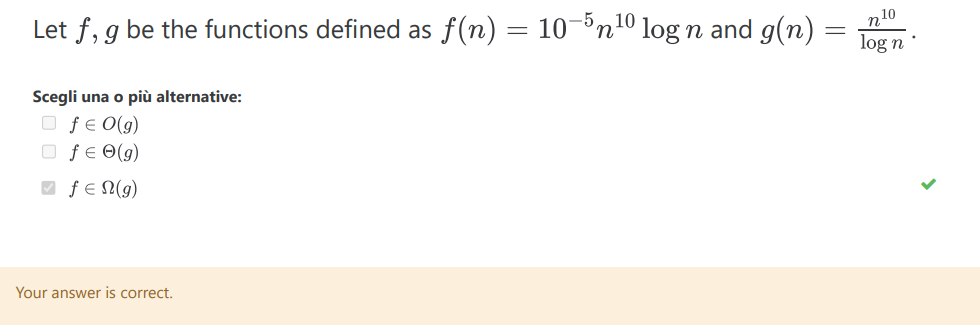
\includegraphics[scale=0.5]{figures/old/theory/15}}
% \end{figure}
%  \begin{figure}[H]
% \centerline{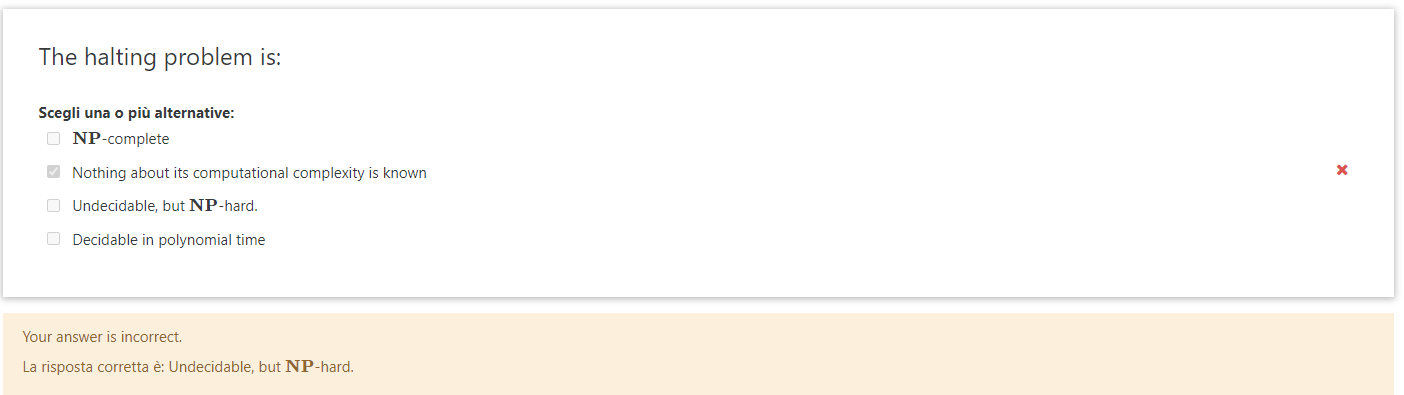
\includegraphics[scale=0.5]{figures/old/theory/16}}
% \end{figure}
%  \begin{figure}[H]
% \centerline{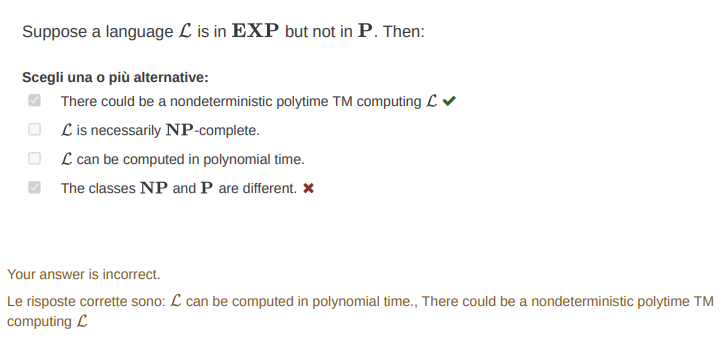
\includegraphics[scale=0.5]{figures/old/theory/17}}
% \end{figure}
%  \begin{figure}[H]
% \centerline{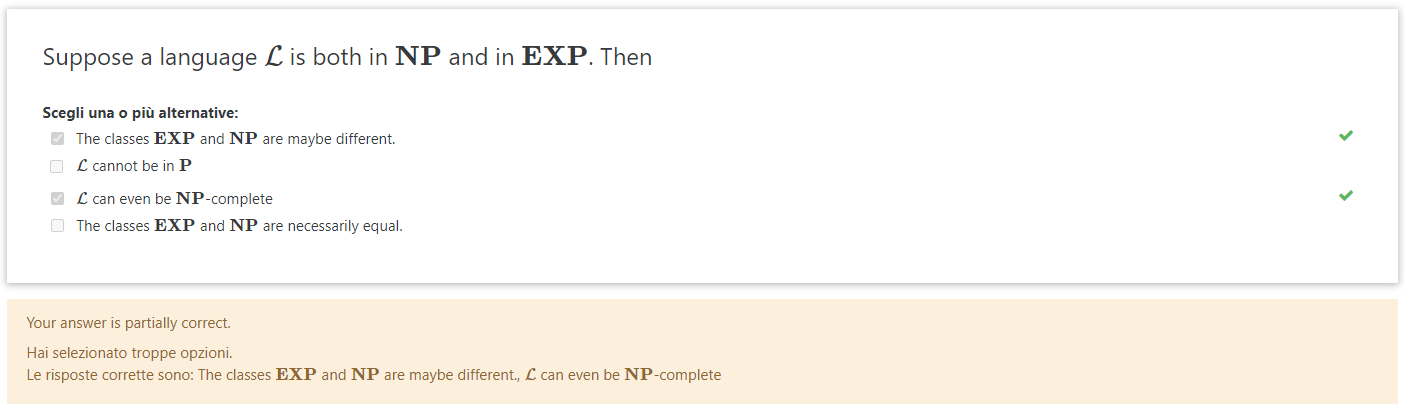
\includegraphics[scale=0.5]{figures/old/theory/18}}
% \end{figure}
%  \begin{figure}[H]
% \centerline{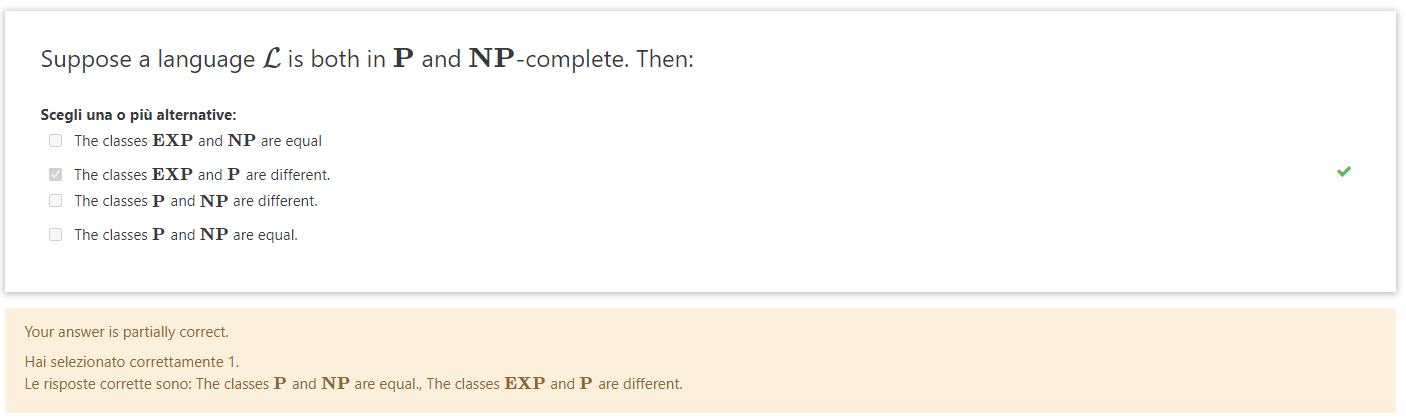
\includegraphics[scale=0.5]{figures/old/theory/19}}
% \end{figure}
%  \begin{figure}[H]
% \centerline{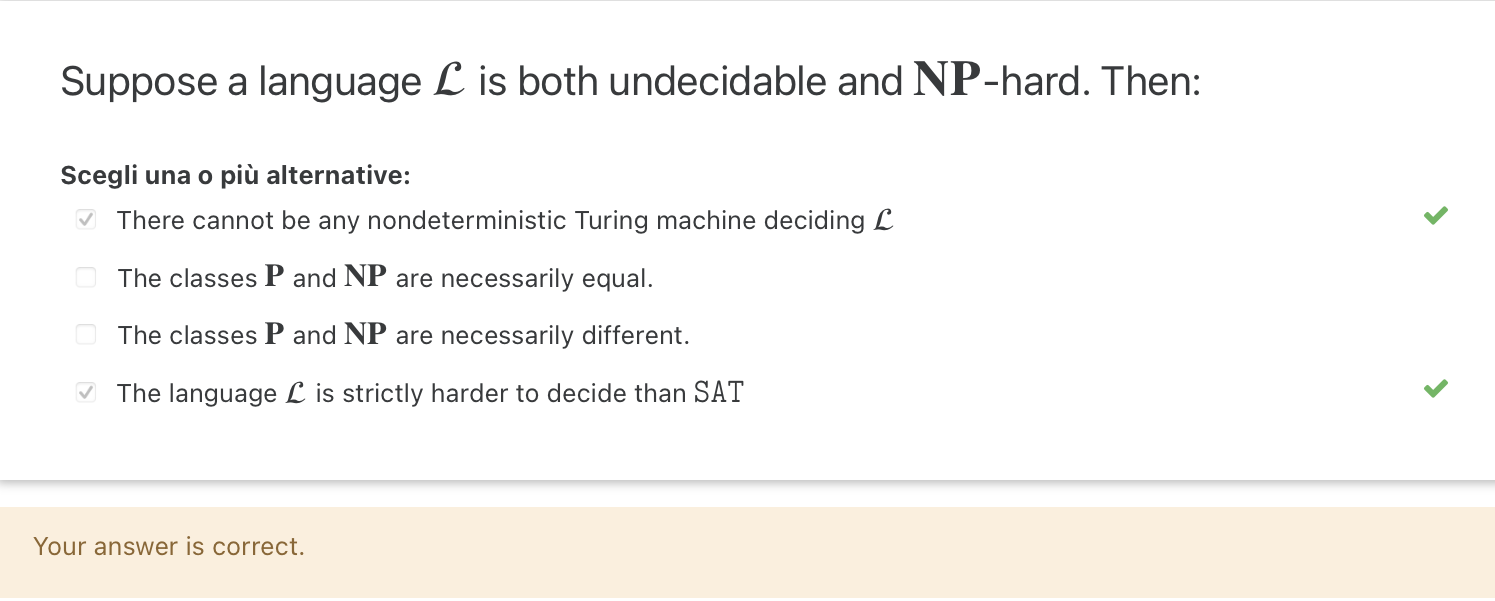
\includegraphics[scale=0.5]{figures/old/theory/20}}
% \end{figure}
%  \begin{figure}[H]
% \centerline{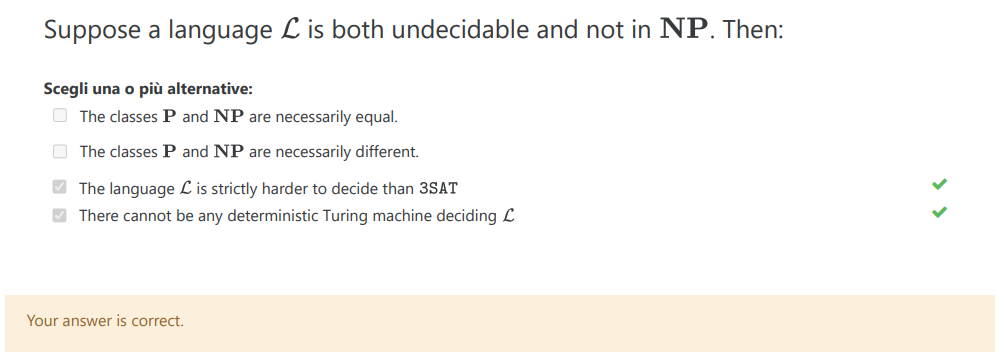
\includegraphics[scale=0.5]{figures/old/theory/21}}
% \end{figure}
%  \begin{figure}[H]
% \centerline{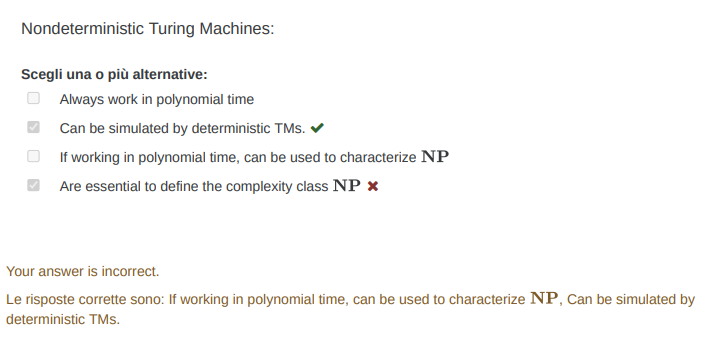
\includegraphics[scale=0.5]{figures/old/theory/22}}
% \end{figure}
%  \begin{figure}[H]
% \centerline{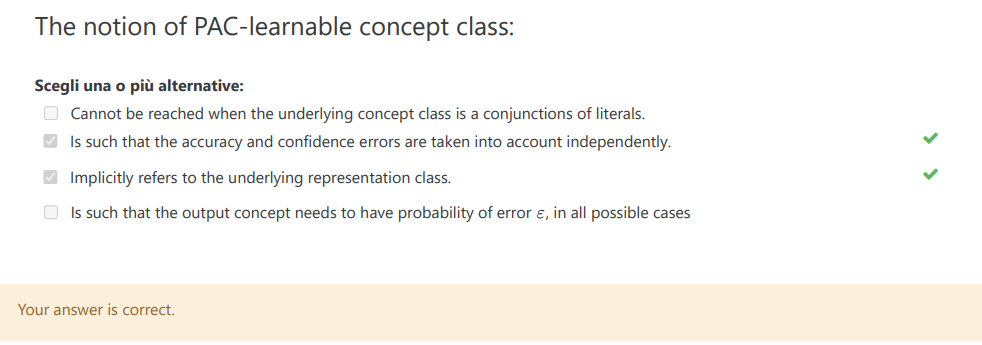
\includegraphics[scale=0.5]{figures/old/theory/23}}
% \end{figure}
%  \begin{figure}[H]
% \centerline{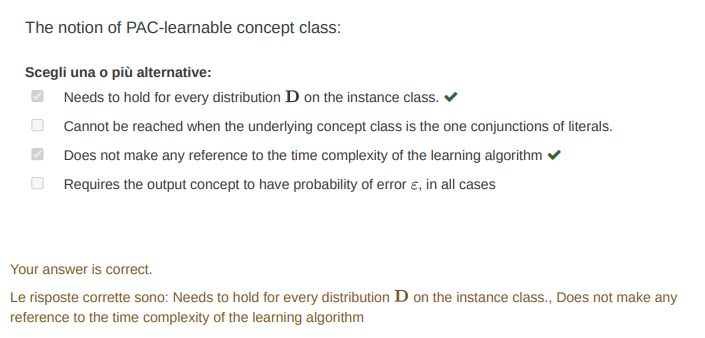
\includegraphics[scale=0.5]{figures/old/theory/24}}
% \end{figure}
%  \begin{figure}[H]
% \centerline{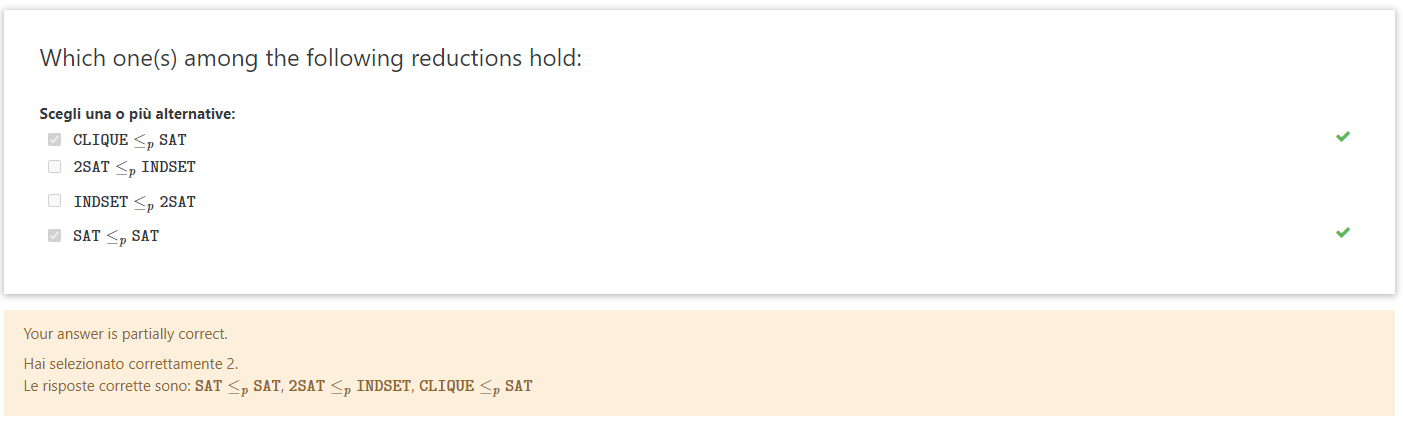
\includegraphics[scale=0.5]{figures/old/theory/25}}
% \end{figure}


